%**************************************************************************************
% License:
% CC BY-NC-SA 4.0 (http://creativecommons.org/licenses/by-nc-sa/4.0/)
%**************************************************************************************

\documentclass[notes]{beamer}

\mode<presentation> {

\usetheme{Madrid}

% Burnt orange
\definecolor{burntorange}{rgb}{0.8, 0.33, 0.0}
\colorlet{beamer@blendedblue}{burntorange}
% Pale yellow
\definecolor{paleyellow}{rgb}{1.0, 1.0, 0.953}
\setbeamercolor{background canvas}{bg=paleyellow}
% Secondary and tertiary palett
\setbeamercolor*{palette secondary}{use=structure,fg=white,bg=burntorange!80!black}
\setbeamercolor*{palette tertiary}{use=structure,fg=white,bg=burntorange!60!black}

% To remove the footer line in all slides uncomment this line
%\setbeamertemplate{footline}
% To replace the footer line in all slides with a simple slide count uncomment this line
%\setbeamertemplate{footline}[page number]

% To remove the navigation symbols from the bottom of all slides uncomment this line
%\setbeamertemplate{navigation symbols}{}
}

\usepackage{amsmath}
\usepackage{bm}
\usepackage{breqn}
\usepackage{cancel}
\usepackage{graphicx} % for figures
\usepackage{subcaption} % for subplots 
\usepackage[labelsep=space,tableposition=top]{caption}
\renewcommand{\figurename}{Fig.} 
\usepackage{cleveref}
\usepackage{caption,subcaption}% http://ctan.org/pkg/{caption,subcaption}
\usepackage{booktabs} % Allows the use of \toprule, \midrule and \bottomrule in tables
\usepackage{multirow}
\usepackage{tabularx}
\usepackage{siunitx}
\usepackage{cleveref}
\usepackage{xcolor}
\usepackage{empheq}
\usepackage[most]{tcolorbox}

\newtcbox{\mymath}[1][]{%
	nobeforeafter, math upper, tcbox raise base,
	enhanced, colframe=blue!30!black,
	colback=blue!30, boxrule=1pt,
	#1}

% To print 2 slides on a page
%\usepackage{handoutWithNotes}
%\pgfpagesuselayout{2 on 1}[border shrink=2mm]
%----------------------------------------------------------------------------------------
%	TITLE PAGE
%----------------------------------------------------------------------------------------
% The short title appears at the bottom of every slide, the full title is only on the title page
\title[CE394M: Tresca \& MC]{CE394M: Tresca and Mohr-Coulomb} 
\author{Krishna Kumar} % name
\institute[UT Austin] % institution 
{
University of Texas at Austin \\
\medskip
\textit{
  \url{krishnak@utexas.edu}} % Your email address
}
\date{\today} % Date, can be changed to a custom date

\begin{document}

\begin{frame}
\titlepage % title page as the first slide
\end{frame}

\begin{frame}
 % Table of contents slide, comment this block out to remove it
 \frametitle{Overview}
  %Throughout your presentation, if you choose to use \section{} and \subsection{} 
  %commands, these %will automatically be printed on this slide as an overview 
 \tableofcontents
\end{frame}

%----------------------------------------------------------------------------------------
% slides
%----------------------------------------------------------------------------------------
\section{Constitutive modeling}
%----------------------------------------------------------------------------------------
\begin{frame}
\frametitle{Stress invariants}
\begin{itemize}
	\item The magnitudes of the component of the stress vector depend on the chosen direction of the coordinate axes (in 3D: 6 variables).
	\item Principal stresses always act on the same planes and have the same magnitude (invariant to the coordinate axes), but still need to define the corresponding orientations (in 3D: 6 variables).
	\item For isotropic materials, it is very convenient to work with alternative invariant quantities which are combinations of principal stresses.
\end{itemize}
\end{frame}

%----------------------------------------------------------------------------------------
\begin{frame}
\frametitle{Stress invariants}
\begin{itemize}
	\item Mean effective stress $p = \frac{1}{3}(\sigma_I + \sigma_II + \sigma_III)$
	\item Deviatoric stress: $J = \frac{1}{\sqrt{6}}\sqrt{(\sigma_I - \sigma_{II})^2 + (\sigma_{II} - \sigma_{III})^2 + (\sigma_{III} - \sigma_I)^2}$
	\item Lode's angle $\theta = \tan^{-1}\left[\frac{1}{\sqrt{3}}\left(2\frac{(\sigma_{II} - \sigma_{III})}{\sigma_I - \sigma_{III}} -1 \right)\right]$
\end{itemize}

Principal stresses can be expressed in terms of invariants:

\begin{equation*}
\begin{bmatrix}
\sigma_I \\
\sigma_{II} \\
\sigma_{III} \\
\end{bmatrix} = 
p \begin{bmatrix}
1 \\
1 \\
1 \\
\end{bmatrix} + 
\frac{2}{\sqrt{3}}J
\begin{bmatrix}
\sin\left(\theta + \frac{2 \pi}{3}\right) \\
\sin \theta \\
\sin\left(\theta - \frac{2 \pi}{3}\right) \\
\end{bmatrix}
\end{equation*}
\end{frame}

\section{Tresca model}
%----------------------------------------------------------------------------------------
\begin{frame}
\frametitle{Tresca model}
Simulation of undrained behavior of saturated clay

Failure criteria: 
\mode<beamer>{
	\begin{equation*}
		\tau_f = s_u
	\end{equation*}
where $\tau_f$ is the shear stress at failure. $s_u$ is the undrained strength.
}
\mode<handout>{
	\vspace{1.5cm}
}
\begin{figure}
	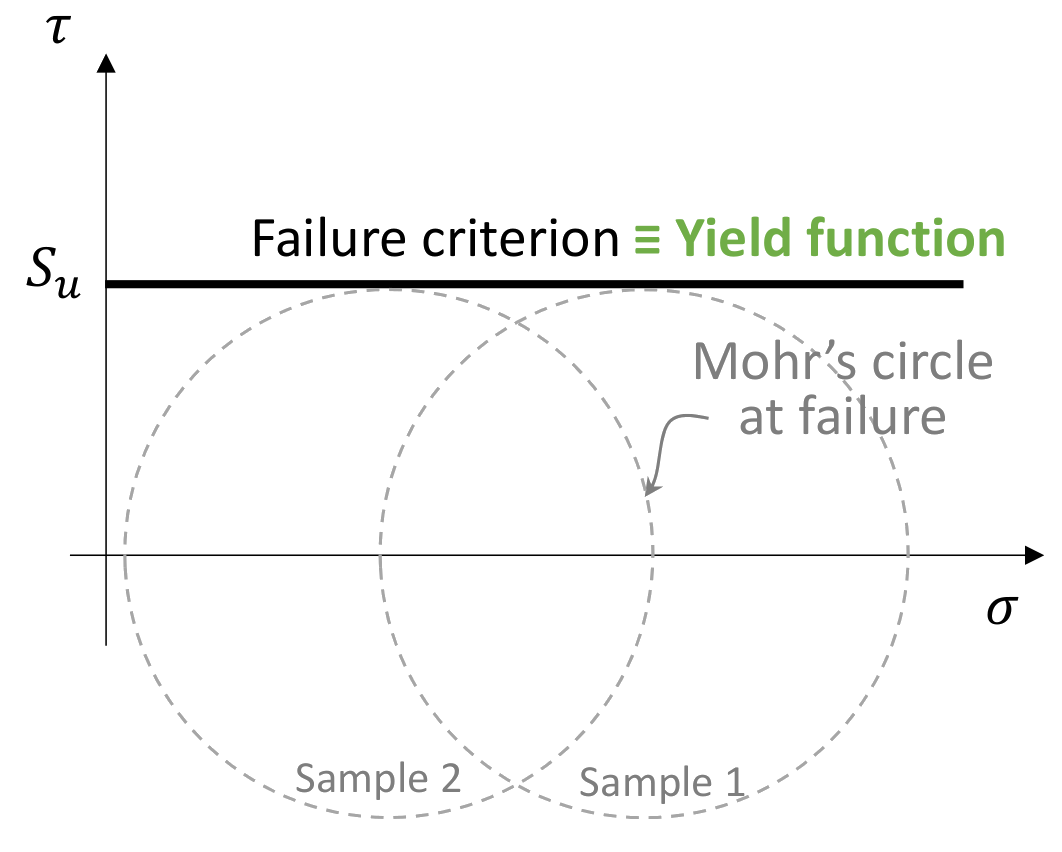
\includegraphics[width=0.55\textwidth]{figs/tresca.png}
\end{figure}
\end{frame}

%----------------------------------------------------------------------------------------
\begin{frame}
\frametitle{Tresca model}
Yield function
\mode<beamer>{
	\begin{align*}
	F (\sigma, W_p) & = \sigma_I - \sigma_{III} - 2 s_u = 0 \\
	& = J \cos \theta - s_u = 0 
	\end{align*}
}
\mode<handout>{
	\vspace{1.5cm}
}
\begin{figure}
	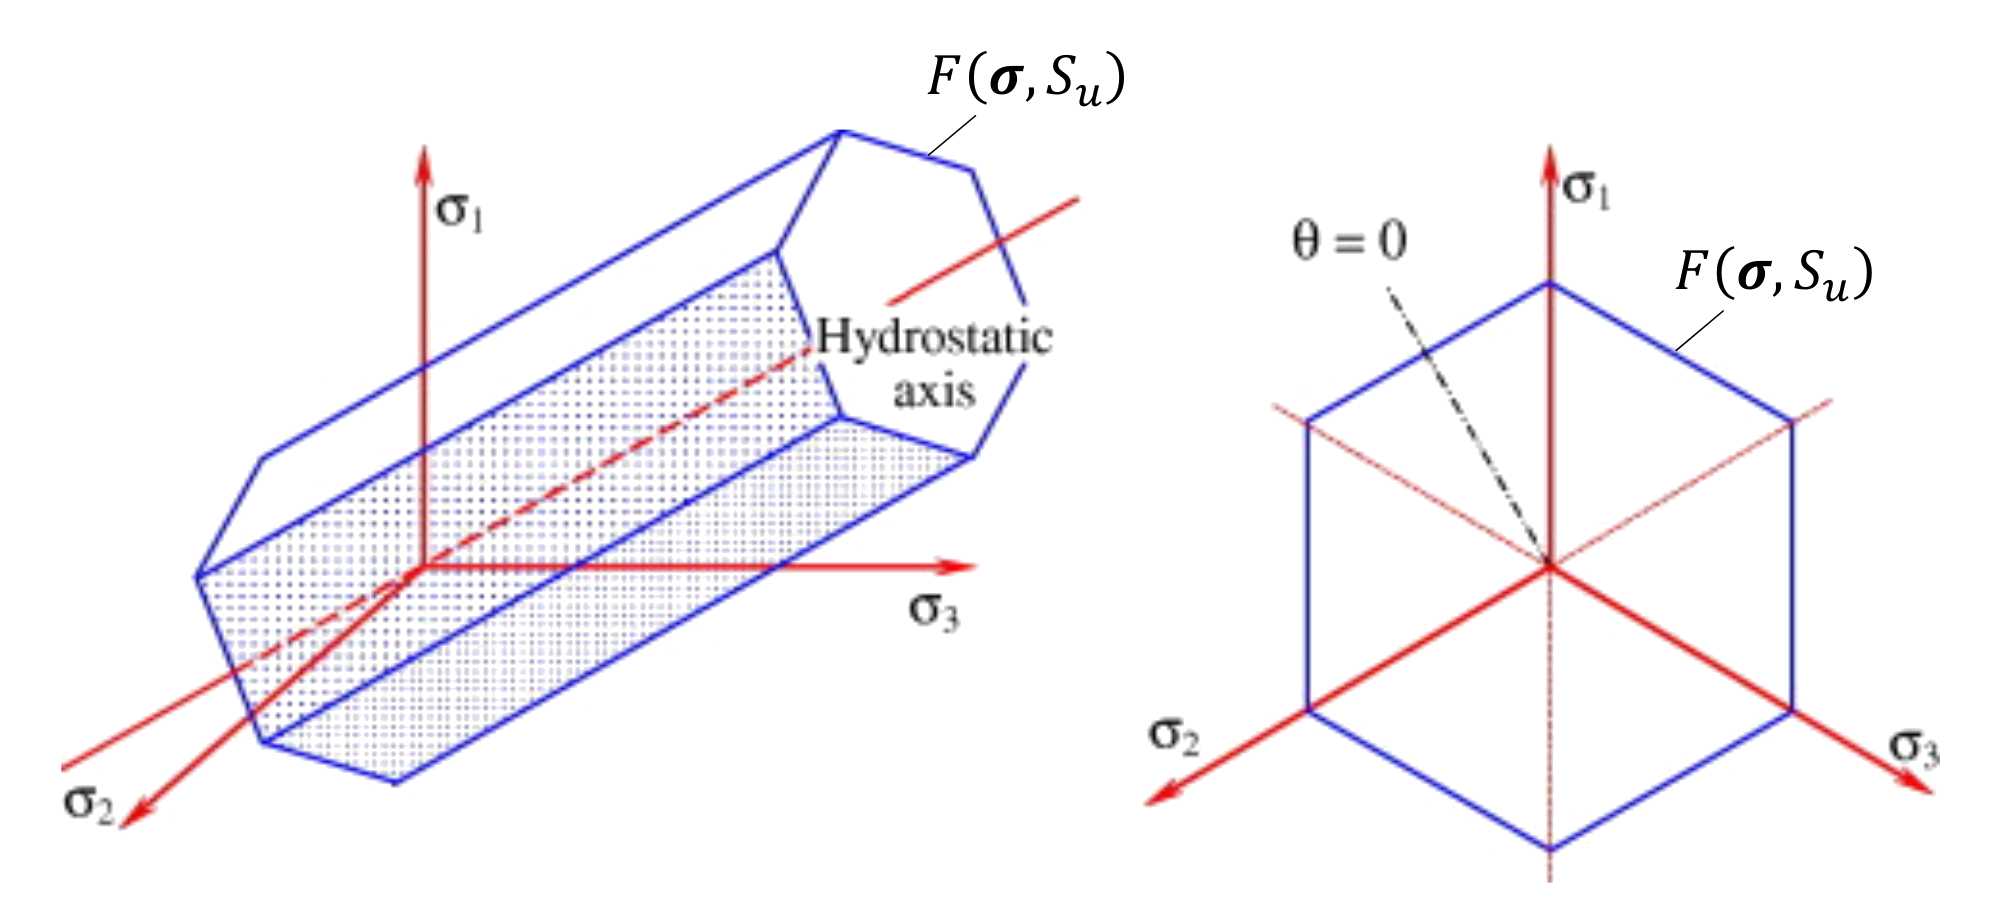
\includegraphics[width=\textwidth]{figs/tresca-yield.png}
\end{figure}
\end{frame}

\end{document}
